\section{Lezione 25 17/11/2023}

\subsection{Dimostrazione Decomposizione di un albero FDF in CC}

Prendiamo per esempio un albero costruito dalla DFS su questo grafo $G$:

\begin{figure}[H]
	\centering
	\begin{subfigure}[b]{0.30\textwidth}
		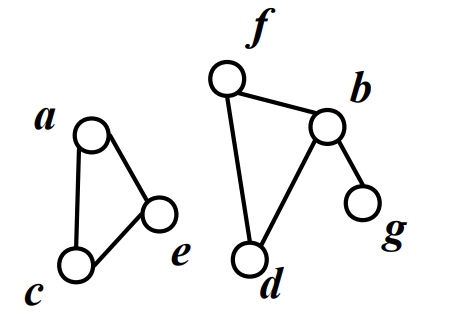
\includegraphics[width=\textwidth]{GrafoConnessoPrimo} 
		%\caption{Grafo non Connesso}
	\end{subfigure}
\end{figure}



Possiamo notare che nell'albero sono presenti 2 Componenti Connesse insieme.\\

\begin{figure}[H]
	\centering
	\begin{subfigure}[b]{0.25\textwidth}
		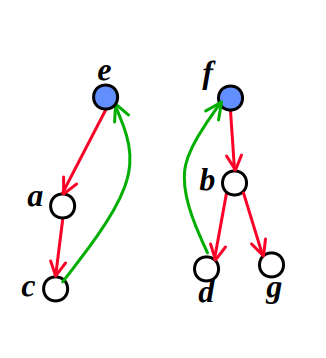
\includegraphics[width=\textwidth]{CFCDoppioLezione25} 
		%\caption{Grafo non Connesso}
	\end{subfigure}
\end{figure}

\paragraph{Ragionamento per Componente Connessa}Possiamo dire che se $u$ e $v \in V$ appartengono alla stessa componente (fortemente) connessa ($C(F)C (u) = C(F)C (v)$), allora ogni percorso da $u$ a $v$ appartiene \textbf{sempre} alla Componente Fortemente Connessa. 

\begin{figure}[H]
	\centering
	\begin{subfigure}[b]{0.30\textwidth}
		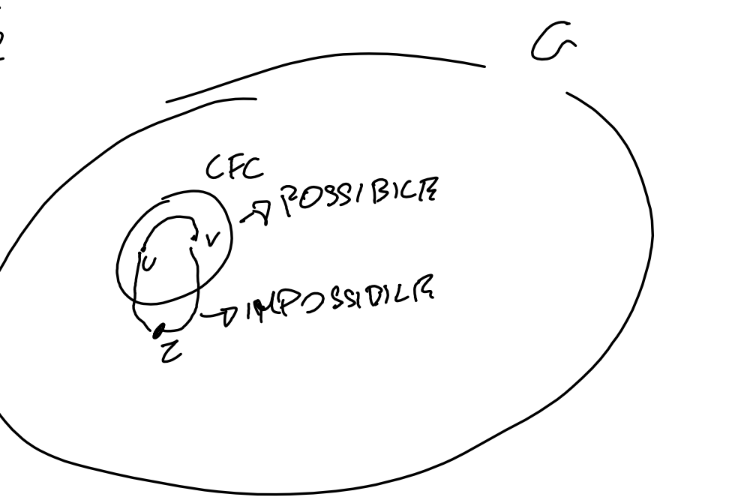
\includegraphics[width=\textwidth]{Lezione25Proprieta1} 
		%\caption{Grafo non Connesso}
	\end{subfigure}
\end{figure}

\paragraph{Dimostrazione}Potremmo dimostrare questa affermazione per assurdo, prendendo un vertice $z$, che non fa parte di $CFC(u)$.\\
 Siccome esiste un percorso da $z$ in $u$, e che sia fortemente connesso per la proprieta di sopra.
 Vedremo che esistera dunque un percorso da $z \rightarrow u$ , ma che essendo fortemente connesso per ipotesi allora, $\exists $ un percorso $u \rightarrow z$, andando a creare un ciclo. E la condizione necessaria per la quale un grafo sia fortemente connesso e la presenza di un ciclo.
 
\begin{figure}[H]
	\centering
	\begin{subfigure}[b]{0.30\textwidth}
		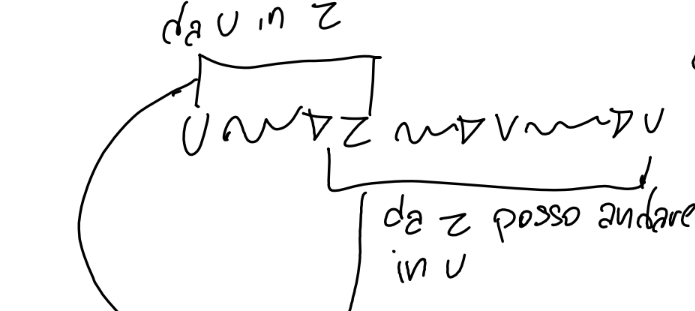
\includegraphics[width=\textwidth]{Lezione25Dimostrazione1} 
		%\caption{Grafo non Connesso}
	\end{subfigure}
\end{figure}


\paragraph{Ragionamento 2}Ora che sappiamo che $u$ e $v$ appartengono alla stessa $C(F)C$, allora possiamo dire che apparterranno allo stesso albero costruito dalla DFS.\\
	
Alla partenza della DFS, l'algoritmo avra mandato nella DFSVisit un nodo radice che prendera il nome di $z$.
Da qui possiamo dare per sicure 2 proprieta:
\begin{itemize}
	\item $z$ sara il primo vertice visitato dalla DFS, ed e anche ovvio.
	\item all'istante $d[z]$, per il teorema del percorso bianco ogni percorso da $z \rightarrow v$ e da $z \rightarrow u$ sono completamente bianchi.
\end{itemize}

	 Dunque arriveremo a dire che :
\begin{itemize}
	 \item I percorsi da $z$ dell'albero sono tutti una $C(F)C$.
	 \item All'istante $d[z]$ i percorsi sono tutti bianchi e per il teorema del percorso bianco, $v$ e $u$ sono discendenti della foresta di $z$.
\end{itemize}

\subsubsection{Come sfruttiamo queste proprieta?}
Nella foresta avremo CFC diverse in una stessa FDF dopo il passaggio della DFS. In ogni FDF c'e una radice che racchiude tutti i nodi di una componente connessa.
Dunque ci basta individuare quali nodi fanno parte della stessa C(F)C, e da quali radici partono quei percorsi per raggiungere i nodi. Dunque potremmo applicare un ragionamento inverso, nella quale dai nodi vorremmo trovare i percorsi che portano alla radice.

%immagine radici diverse in FDF uguali%

%foto%

Nel nostro esempio, nella prima parte del grafo, i 3 nodi $a,c,e$ raggiungono la stessa radice, mentre per l'altra parte del grafo:
%foto%

I nodi $b,d$ riescono a raggiungere senza problemi la nostra radice $f$, mentre g no.

\subsubsection{Il Grafo Trasposto}

Per ovviare a problemi del genere possiamo creare un \textbf{Grafo Trasposto} $G^{T}$ costruito in questo modo:\medskip

Se in $G \exists \pi: u \rightarrow v $, allora $G^{T} \exists \pi^{\prime}: v \rightarrow u$ e viceversa. Quindi un grafo le cui direzioni degli archi sono completamente invertite.

%foto del grafo invertito%

\paragraph{Soluzione}	La proprieta che prende questo grafo invertito e che ci servira per la definizione delle C(F)C e che se ogni percorso dalla radice $r$ arriva ai suoi vertici $v$ nell'albero FDF e ogni vertice $v$ nel grafo $G^{T}$ arriva a $r$, allora potremmo ipotizzare che ogni vertice del grafo faccia parte della stessa $C(F)C(r)$. 



\paragraph{Problema}
	Il nostro ragionamento funziona a patto che la DFS sappia di doversi fermare all'interno della stessa C(F)C.

Infatti se dovessimo ricostruire l'albero creato dalla DFS nel grafo trasposto, osserveremo che invece di dividere ancor di piu le C(F)C, ha unito tutto il grafo.

%Le due foto a paragone qua%

Il problema di questo ragionamento e stato solamente la presenza di un \textbf{arco di attraversamento}, che ha unito, nel grafo trasposto, i 2 sottografi, e che, al passaggio della DFS, ha permesso di aggiungere tutti i rimanenti nodi nello stesso albero FDF.

\subsubsection{La soluzione agli archi di attraversamento}

Se ragioniamo su come funzionano gli archi di attraversamento, vedremo che ognuno di esse connette alberi creati dalla DFS sempre in una stessa direzione. La direzione che prende ha lo stesso verso del \textbf{tempo} che impiega la DFS a compiere le sue funzioni. Quindi in poche parole gli archi di attraversamento hanno tutti uno stesso verso.

\paragraph{Ragionamento}
	Nel caso in cui dunque ci troviamo nell'ultimo albero da visitare, non esisteranno archi di attraversamento, quindi la visita DFS sulla $k$-esima radice dell'albero raggiungera vertici contenuti solamente nell'albero creato da $k$.
	In effetti allora, questi stessi vertici andranno a creare la CFC($r_k$).


%foto%


\paragraph{Idea}Dunque potremmo utilizzare questa nozione per trovare il modo di "ragionare a ritroso" e selezionare soltanto quei vertici da mandare poi in DFSVisit (Per il grafo inverso) in un certo ordine.

\subsection{La soluzione per i grafi orientati}

Dunque gli step per riuscire a trovare queste C(F)C sono i seguenti:

\begin{itemize}
	\item Fare una DFS su $G$ normalmente ma salvarsi le radici in uno stack.


\begin{lstlisting}[language=Java]
	DFSVariante(G)
		Init(G)
		For Each $v \in V$ do
			if col[v]=b then
				S=DFSVisitVariante(G,v,S)//dove S e uno stack vuoto che viene riempito a ogni radice di sottoalbero
\end{lstlisting}


\begin{lstlisting}[language=Java]
	DFSVisitVariante(G,v,S)
		col[v]=G
		For Each $u \in Adj[v]$ do
			if col[u] $\neq$ b then
				S = DFSVisitVariante(G,u,S)
		S=Push(S,v)
		Col[v]=n
		return S
\end{lstlisting}

\newpage

\item Fare una seconda DFS (modificata) su $G^{T}$ e selezionando le radici in ordine inverso, cioe dal tempo piu lontano di visita al piu vicino.

\begin{lstlisting}[language=Java]
	$DFS^{\prime}$($G^{T}$,S)
		Init($G^{T}$)
		While S $\neq \varnothing$ do
			v = Top(S)
			if Col[v] = b then
				$DFS{\prime}$Visit($G^{\prime}$,v)
			S = Pop(S)
\end{lstlisting}

\begin{lstlisting}[language=Java]
	$DFS^{\prime}$Visit($G^{\prime}$,v)
		col[v]=g
		For Each u $\in$ Adj[v] do
			if col[v]=b then
				pred[u]=v
				$DFS^{\prime}$Visit($G^{\prime}$,u)
\end{lstlisting}
	
\end{itemize}

\subsubsection{Algoritmo CFC}

L'algoritmo C(F)C che regola appunto queste funzioni che abbiamo creato sopra e il seguente:


 \begin{lstlisting}[language=Java]
 		CFC(G)
 			s=DFS(G)
 			$G^{T}$=Trasposta(G)
 			$DFS^{\prime}$($G^{T}$,S)
 \end{lstlisting}

Questo algoritmo racchiude le funzioni per trovare le componenti fortemente connesse di un grafo.

Al termine di questo algoritmo ogni albero della seconda DFS contiene tutti e soli i nodi della C(F)C($v$) dove $v$ e la radice dell'albero formato, senza incorrere in problemi come arco trasposto.

\subsubsection{Il costo dell'algoritmo}

Il costo della creazione del grafo trasposto e da calcolare:
\begin{lstlisting}[language=Java]
	Trasposto(G)
		$V^{T}$ = NIL
		For Each v $\in$ V do
			$V^{T}$=$V^{T} \cup \{v\}$
		For Each $v \in$ V do
			For Each $u \in$ Adj[v]
				$Adj^{\prime}$[u] = add($Adj^{\prime}$,v)//liste dinamiche 
		return ($V^{T}$, $Adj^{T}$[u])
\end{lstlisting}

Questo algoritmo di so occupa di scorrere tutte le liste di adiacenza di ogni vertice e invertire l'arco.

\subsection{Esempio}

%Lezione25EsempioFinale1
\begin{figure}[H]
	\centering
	\begin{subfigure}[b]{0.40\textwidth}
		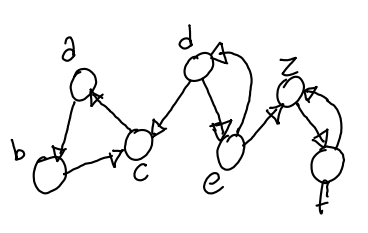
\includegraphics[width=\textwidth]{Lezione25EsempioFinale1} 
		%\caption{Grafo non Connesso}
	\end{subfigure}
\end{figure}
Dato questo grafo, vogliamo provare a trovare le sue componenti fortemente connesse. Dunque, come abbiamo detto andiamo ad eseguire la DFS(a) e la DFS(d) (Partiamo con il primo vertice del grafo $a$ e continuiamo con il primo non visitato in ordine alfabetico $d$), visto  che con una DFS non si riesce a visitare tutto l'albero.

\begin{figure}[H]
	\centering
	\begin{subfigure}[b]{0.40\textwidth}
		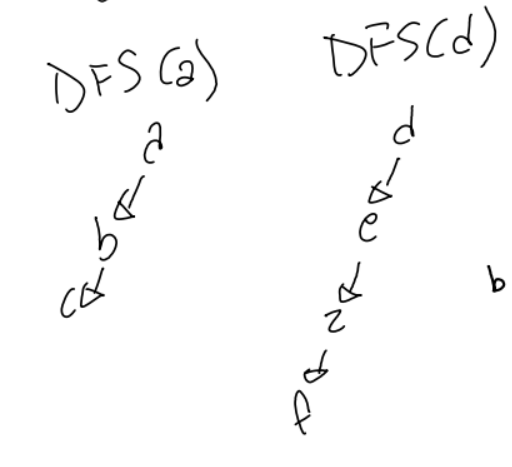
\includegraphics[width=\textwidth]{Lezione25Esempio2.png} 
		%\caption{Grafo non Connesso}
	\end{subfigure}
\end{figure}

Durante questo processo di DFS, andiamo a prenderci ogni vertice della DFSVisit', che corrisponde a ogni vertice dell'albero di adiacenti creato, in ordine di visita. In particolare andremo ad inserire (Push) dal primo vertice che viene terminato (f[c]) all'ultimo (f[d]) dato che f[d]>f[c].


\begin{figure}[H]
	\centering
	\begin{subfigure}[b]{0.20\textwidth}
		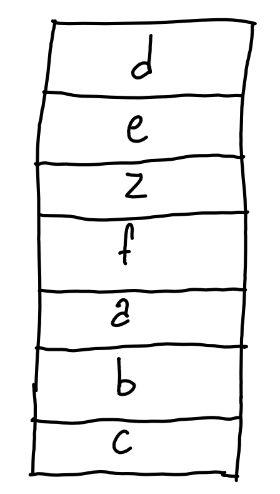
\includegraphics[width=\textwidth]{Lezione25Esempio3.png} 
		%\caption{Grafo non Connesso}
	\end{subfigure}
\end{figure}

Dopodichè andiamo a costruire il grafo trasposto grazie alla nostra funzione di trasposizione.

\begin{figure}[H]
	\centering
	\begin{subfigure}[b]{0.40\textwidth}
		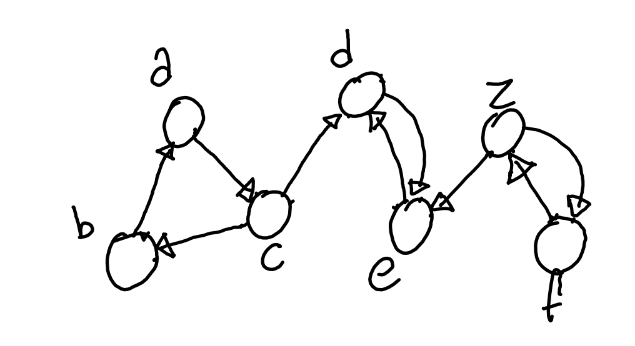
\includegraphics[width=\textwidth]{Lezione25Esempio4.png} 
		%\caption{Grafo non Connesso}
	\end{subfigure}
\end{figure}

A questo punto prendiamo dallo stack da noi creato il primo elemento e da li creiamo la DFS, continuamo cosi finchè lo stack non diventa vuoto.
A quel punto come vedremo avremo creato i nostri alberi C(F)C, come da foto qui sotto.

\begin{figure}[H]
	\centering
	\begin{subfigure}[b]{0.30\textwidth}
		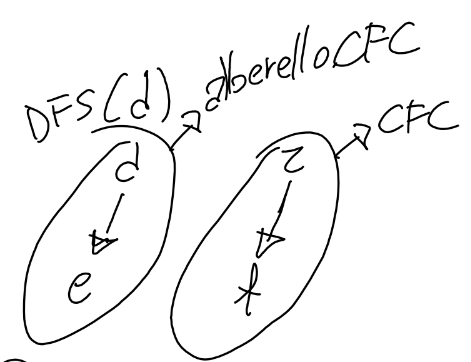
\includegraphics[width=\textwidth]{Lezione25Esempio5.png} 
		%\caption{Grafo non Connesso}
	\end{subfigure}
\end{figure}

\begin{figure}[H]
	\centering
	\begin{subfigure}[b]{0.25\textwidth}
		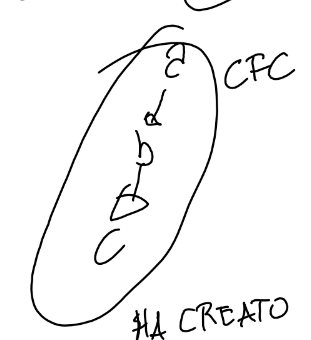
\includegraphics[width=\textwidth]{Lezione25Esempio6.png} 
		%\caption{Grafo non Connesso}
	\end{subfigure}
\end{figure}